\section{METODOLOGIA}
    % apresentação da metodologia utilizada para a resolução do problema, descrição dos dados utilizados, e descrição dos métodos de otimização utilizados, além do método científico utilizado para a resolução do problema
    
    \ipar O método de pesquisa aplicado neste estudo é de pesquisa de modelagem quantitativa baseado em modelo empírico. Este tipo de modelagem descritiva busca identificar o melhor ajuste dentre as observações e atuar em modelos reais, desta forma, a pesquisa contempla uma validação do constructo dos modelos científicos baseando em pesquisas teóricas quantitativas \cite{bertrand2002operations}.

    \ipar A metodologia está dividida em algumas etapas: coleta de dados, pré-processamento, modelagem de dados, otimização de portfólio, treinamento de redes neurais e validação de modelos.

    \subsection{Coleta de dados}
        % Fonte de dados, forma de obtenção, limitações definidas, justificativa da escolha dos dados, e descrição dos dados utilizados (preços, índices, indicadores, e dados de corretores). Criação de métodos de automação de coleta de dados.

        \ipar Os dados utilizados neste estudo são dados públicos, disponibilizados gratuitamente por instituições financeiras e órgãos governamentais. Os dados são coletados através de códigos de programação que acessam diretamente as fontes oficiais. Para o desenvolvimento deste estudo, uma ferramenta de automação para atualização automática dos dados diariamente foi elaborada e integrada a uma plataforma de mensagens instantâneas, desta forma, os dados são atualizados mediante requisição e armazenados localmente.

        \ipar Utilizou-se dados de preços de ativos, índices de mercado e indicadores econômicos. Os dados de preços de ativos e os dados de índices de mercado são coletados diretamente da \acrshort{B3} (\acrlong{B3}), a bolsa de valores do mercado brasileiro. Os dados de indicadores econômicos são coletados diretamente do Banco Central do Brasil \cite{bcb2023selic}.
        
        \ipar A delimitação das séries históricas utilizadas neste estudo para coleta de dados é de 01/07/1994 até 31/05/2023, com intervalo de 1 dia útil. A escolha desta delimitação, dá-se pela estabilidade da economia brasileira após o plano real. Entretanto, o indicador econômico de taxa de juros SELIC, tem valor referencial a partir de 01/07/1996, além disso, o indicador de mercado \acrshort{IBOVESPA} tem valor referencial a partir de 02/01/1998. Desta forma, os dados de preços de ativos e índices de mercado são estruturados a partir da última data de referência dos indicadores econômicos.

        \ipar A escolha do índice de mercado \acrshort{IBOVESPA} como referência para o mercado brasileiro se dá pela sua representatividade, pois o índice é composto pelas ações mais negociadas na bolsa de valores brasileira, além disso, o índice é utilizado como referência para diversos fundos de investimentos e carteiras de investimentos. A escolha do indicador econômico de taxa de juros SELIC como referência se dá pela sua representatividade, pois a taxa é utilizada como referência para diversos investimentos de renda fixa, para diversos fundos e carteiras de investimentos. Esta taxa é utilizada como referência para a taxa livre de risco.

        \ipar Os ativos financeiros, objeto de estudo, são os componentes do índice de merca-do \acrshort{IBOVESPA} no intervalo delimitado, pois são ativos previamente avaliados pelos critérios do índice, e portanto são ativos de maior liquidez e representatividade no mercado brasileiro. Os ativos financeiros são ações ordinárias e preferenciais, fundos imobiliários, e fundos de investimentos em ações, além disso, os ativos financeiros são classificados em ativos de renda variável.

        \ipar Informações cadastrais dos ativos financeiros são coletadas diretamente da B3, incluindo nome, código, tipo e setor do ativo, além do tamanho de lote mínimo e valor de mercado. Informações cadastrais dos ativos financeiros são utilizadas para filtrar ativos financeiros, e para cálculo de custos operacionais. Por outro lado, informações relevantes das séries históricas, como desdobramentos e grupamentos, são coletadas via \textit{Yahoo Finance}, sendo utilizadas para o cálculo de preços ajustados, pois os dados obtidos da B3 demonstraram inconsistências quanto a estes eventos.

        \ipar As corretoras praticam diversas taxas e custos operacionais, entretanto, para este estudo, considera-se taxa de corretagem, sendo a taxa cobrada pela corretora para cada operação de compra e venda de ativos financeiros, e também considera-se taxa de custódia, que é a taxa cobrada pela bolsa de valores brasileira para manter os ativos financeiros em custódia. As taxas de corretagem e custódia são coletadas diretamente das corretoras, e são utilizadas para cálculo de custos operacionais. Adiciona-se também o imposto de renda, sendo a taxa cobrada pelo governo brasileiro sobre o lucro de operações de compra e venda de ativos financeiros.

        \ipar Os dados coletados são armazenados em arquivos de formato CSV e formato hierárqui-co de dados (do inglês, \textit{Hierarchical Data Format} (HDF5)), organizados em pastas de acordo com o tipo de dado e nomeados conforme o tipo e a data de referência. O quadro \ref{quadro:coleta_dados} apresenta os dados coletados, a fonte e a descrição destes dados.

        \begin{quadro}[htp]
            \centering
            \caption{Dados coletados}
            \label{quadro:coleta_dados}
            \begin{tabular}{lll}
                \hline
                \textbf{Dados} & \textbf{Fonte} & \textbf{Descrição} \\ \hline \hline
                Preços de ativos & B3 & \begin{tabular}[c]{@{}l@{}}Preços diário de ativos financeiros \\ negociados na B3\end{tabular} \\ \hline
                Índice Bovespa & B3 & \begin{tabular}[c]{@{}l@{}}Índice de mercado diário calculado \\ pela B3\end{tabular} \\ \hline
                Componentes do Ibovespa & B3 & \begin{tabular}[c]{@{}l@{}}Lista de ativos financeiros componentes \\ do Ibovespa\end{tabular} \\ \hline
                Informações cadastrais de ativos & B3 & \begin{tabular}[c]{@{}l@{}}Informações cadastrais no dia dos ativos \\ financeiros listados na B3 \end{tabular} \\ \hline
                Taxa SELIC & Banco Central & \begin{tabular}[c]{@{}l@{}}Taxa de juros anual por dia pelo Banco \\ Central\end{tabular} \\ \hline
                Taxas de corretagem & Corretora & \begin{tabular}[c]{@{}l@{}}Taxas de corretagem cobradas pelas\\ corretoras\end{tabular} \\ \hline
                Taxas de custódia & Corretora & \begin{tabular}[c]{@{}l@{}}Taxas de custódia cobradas pela B3 \\ \end{tabular} \\ \hline
                Imposto de renda & Receita Federal & \begin{tabular}[c]{@{}l@{}}Tabela de alíquotas de imposto de renda \\ por tipo de ativo\end{tabular} \\ \hline
                Desdobramentos e grupamentos & \textit{Yahoo Finance} & \begin{tabular}[c]{@{}l@{}}Desdobramentos e grupamentos de \\ ativos financeiros\end{tabular} \\ \hline
            \end{tabular}
            \par \footnotesize Fonte: próprio autor.
        \end{quadro} 


        \ipar Como o volume de dados coletados é grande, e o tempo de coleta é longo quando realizado manualmente, a coleta de dados é automatizada através de códigos de programação, permitindo a atualização diária dos dados mediante requisição. Os códigos de programação estão disponíveis no repositório do projeto, e uma peça do código é exemplificada no apêndice A.

    \subsection{Pré-processamento de dados}
        % Filtros aplicados aos preços, tratamento de dados faltantes, tratamento de outliers, correção de splits, conversão de valores anuais para diários e precificado, definições de janelas de tempo, definição de intervalos, tratamento de início e fim de intervalos, definição de taxa livre de risco para intervalo, concatenar dados e tratamento de faltantes. Criação de métodos de automação de tratamento de dados. 

        \ipar Como os dados têm origem de diversas fontes e não são padronizados, isto é, possuem diferentes estruturas e formatos, os dados são pré-processados para a aplicação nos modelos de otimização e treinamento de redes neurais. O pré-processamento é realizado para garantir o paralelismo de informações, e assim seguindo para filtragem por parâmetros definidos, tratamento de dados faltantes, tratamento de valores atípicos, conversão de valores e de intervalos, para, enfim, compor uma única base concatenada de dados.
.

        \ipar Os preços de ativos da base de dados, contém informações de todos os produtos financeiros negociados pela bolsa de valores no período considerado, sendo necessária a filtragem para selecionar apenas os ativos de interesse e os valores de fechamento do dia. Os ativos de interesse deste estudo são os componentes do índice Bovespa na data de referência. Um módulo foi elaborado para permitir a seleção de ativos de interesse, e a filtragem de ativos com base em parâmetros definidos, tal qual, o uso de uma lista predeterminada de ativos, ou pelo total de negociações por um intervalo de tempo.

        \ipar Com os preços de fechamento dos ativos, uma etapa de ajuste de valores atípicos é realizada. Esta etapa considera os ajustes de desdobramentos e agrupamentos para que os valores de fechamento sejam corrigidos considerando as devidas proporções. Neste estudo, o ajuste de valores pagos de dividendos não é realizado, pois a fonte de dados de dividendos não demonstrou consistência para aplicação. 

        \ipar No tratamento dos dados, é observado dados faltantes nas séries de preços. Portanto, os dados faltantes para os preços de fechamentos são interpolados entre os valores anteriores e posteriores a este dado faltante. Não é realizada a operação para os valores anteriores ao início da série temporal do próprio ativo, casos de ativos que tiveram a oferta inicial de ações após o início da série temporal.

        \ipar A taxa de juros, SELIC, é convertida a partir de dados diários de taxa anual, para dados diários de taxa diária, considerando 365 dias úteis no ano e precificado em unidades monetárias. O índice Bovespa tem sua pontuação utilizada tal qual é disponibilizada pela B3, sem ajustes de valores atípicos, ou de valores faltantes. Desta maneira, a taxa de juros e o índice Bovespa são concatenados com os preços de fechamento dos ativos. Quando avaliados os dados em paralelo, os períodos que possuam valores faltantes são descartados para a análise para todos os ativos. O fluxo de pré-processamento de dados é apresentado na Figura \ref{fig:fluxo_preprocessamento}.

        \begin{figure}[htp]
            \centering
            \caption{Fluxo de pré-processamento de dados}
            \label{fig:fluxo_preprocessamento}
            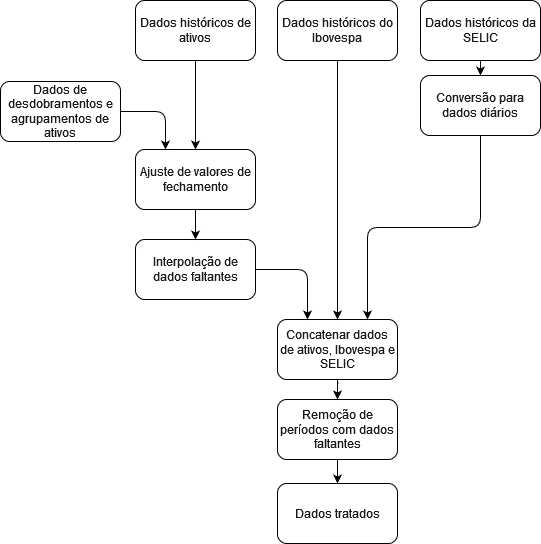
\includegraphics[width=0.9\textwidth]{imagens/fluxo_tratamento.png}
            \par \footnotesize Fonte: próprio autor.
        \end{figure}

        \ipar Todas as etapas do pré-processamento de dados são realizadas por códigos de progra-mação, permitindo a automatização desse processo. Os códigos de programação estão disponíveis no repositório do projeto, e uma peça do código é exemplificada no apêndice A.

    \subsection{Modelagem de dados}
        % Cálculos de ativos, para retornos com médias simples, médias móveis, médias móveis exponenciais, médias móveis autorregressivas, e médias móveis integradas autorregressivas. para risco, variância, VaR, CVaR, ARCH, GARCH. Para correlação, covariância e correlação de Pearson, correlação condicional constante, e correlação condicional dinâmica. Criação de métodos de automação de modelagem de dados. tratamento de dados faltantes, ajustes de intervalos, e definição de janelas de tempo, definição de inicio. Desenvolvimento de métodos de automação de modelagem de dados.

        \ipar Com os dados pré-processados, os dados são modelados para a aplicação na otimização e treinamento de redes neurais. Os dados são modelados para o cálculo de retornos, riscos e correlações, e por fim para compor uma única base de dados para as etapas seguintes.

        \ipar Os parâmetros para o cálculo do retorno, risco, e matriz de covariância dos ativos são o método de cálculo da média, variância e correlação, o intervalo temporal, o tamanho do intervalo, e se os dados já estão filtrados.
        
        \ipar Com a entrada dos dados tratados, dado o intervalo temporal desejado, é feita a modifi-cação dos dados para serem diários, semanais, mensais, trimestrais, semestrais ou anuais. Além disso, é possível definir se a referência temporal é o início ou o final do intervalo, ou seja, se dentro do intervalo a data de referência inicial é o início da semana, mês ou outro, ou se é a última data diária dentro do intervalo. Após a definição do intervalo temporal, o filtro do período de tempo é realizado, e os dados são agrupados conforme o intervalo temporal definido, como exemplo semanal ou mensal. Portanto, define-se a unidade de tempo e o período de análise, como exemplo, filtra-se dados de início de semana a partir de 2018 por 60 semanas, e os dados são agrupados por semana, ou seja, o primeiro dia da semana será a referência para o filtro dos dados, e são selecionados os valores das datas obtidas. 

        \ipar Após o agrupamento dos dados, verifica se já havia algum tratamento prévio de seleção de período, para definir se o intervalo de análise coincide com o intervalo do parâmetro, assim os ativos que apresentarem valores faltantes durante o período selecionado são descartados. Isto ocorre devido ao lançamento do ativo posterior a data de início de análise, portanto, o ativo não apresenta dados suficientes para os cálculos seguintes.

        \ipar Com os dados filtrados, é feito o cálculo dos retornos, riscos e correlações dos ativos após o cálculo de retorno diário por diferença percentual. O retorno esperado dos ativos é calculado com base no método definido, sendo dentre estes, a média simples, médias móveis, médias móveis exponenciais, ARIMA(0,1,1). Os riscos são calculados com base no método de desejado para definição da variância, sendo estes o desvio padrão e GARCH(1,1). As correlações são calculadas na série temporal e aplicadas no cálculo da covariância.

        \ipar A modelagem gera \textit{dataframes} com os dados tratados para o período e intervalo defini-do, um \textit{dataframe} com os retornos, outro com os riscos, e outro com as covariâncias. Os cálculos são realizados por meio de códigos de programação, permitindo a automatização do processo de modelagem de dados. Os códigos de programação estão disponíveis no repositório do projeto.

        \ipar Assim, um módulo é desenvolvido onde são preparadas combinações de intervalos de tempo (diários, semanais e mensais) com métodos para cálculo de risco e retorno para serem inseridas na etapa seguinte de otimização de portfólios. Os intervalos de tempo são definidos como diários, semanais e mensais, e os métodos de cálculo de risco e retorno são definidos como média simples, médias móveis, médias móveis exponenciais, ARIMA(0,1,1), desvio padrão e GARCH(1,1).

        \ipar Todas as etapas da modelagem de dados são realizadas por códigos de programação que estão disponibilizados no repositório do projeto.

    \subsection{Otimização de portfólio}
        % Cálculo de otimização de portfólio, com base no índice sharpe, var e cvar, com váriaveis relaxadas, com aplicação de capital e preço de ativos, com aplicação de lotes mínimos, com aplicação de restrição de aceitação ao risco, com rebalanciamento, com restrição de total de ativos na carteira, e custos operacionais. Aplicação de heurística para otimização de portfólio BKS, relaxação das variáveis e ordenação de ativos. Resultado de distribuição de ativos, e resultados de otimização de portfólio. Criação de métodos de automação de otimização de portfólio.

        \ipar Com os dados modelados e os parâmetros definidos, é realizada a otimização de portfó-lios. O objetivo é definir a alocação ótima de ativos. A base para cálculo considera a série temporal definida, o retorno esperado dos ativos, matriz de covariância e a taxa livre de risco para a otimização de carteira para o método com índice Sharpe dado pela equação \ref{eq:sharpe}. O método utiliza variáveis de decisão de proporção simples dos ativos. Este modelo considera que as variáveis possuem distribuição normal, e que o retorno esperado é a média dos retornos, e o risco é a variância dos retornos.
        
        \ipar Como a função objetivo é não-linear, utiliza-se o método de programação sequencial quadrática para a solução do problema. A biblioteca de otimização \textit{scipy.optimize} do Python contém um módulo de programação sequencial quadrática, portanto este módulo é utilizado para a solução do problema. O módulo de otimização da biblioteca é baseado no modelo de \citeonline{kraft1988sqlsp}.
        
        \ipar As ferramentas de otimização para programação não linear são susceptíveis a mínimos locais, isto é, o algoritmo encontra um mínimo que pode não ser o mínimo global. Portanto, o método é dependente da escolha do ponto inicial. Uma solução, é a escolha aleatória do ponto inicial com a utilização de uma distribuição de probabilidade multivariada contínua, especificamente a distribuição de Dirichlet, no qual gera um vetor não nulo para variável de decisão, e a soma dos elementos do vetor é igual a 1. Logo, a distribuição de Dirichlet é utilizada neste estudo para gerar o ponto inicial. A biblioteca \textit{NumPy} do Python possui a função \textit{random.dirichlet} para geração de amostras da distribuição de Dirichlet.

        \ipar Quando se trata de parâmetros reais, a otimização se torna mais complexa, sendo necessários métodos para solução com técnicas específicas para otimização de valores inteiros. Assim, são adicionados aos modelos as restrições quanto a capital, o preço do ativo, o lote padrão de compra, a quantidade mínima e máxima de lotes, os custos de operação com taxas e impostos, a aceitação ao risco, o rebalanceamento, e quantidade máxima de ativos na carteira. Para construção de uma carteira ótima considerando parâmetros reais, é necessário elaborar um modelo matemático. Para o modelo, é proposto a aplicação das seguintes restrições: capital de investimento, custos de operação, cotação e lotes de negociação, rebalanceamento, aversão ao risco e somente posições de compra. A equação \refeq{eq:otimizacao} apresenta o modelo matemático proposto neste estudo.

        \begin{subequations}
            \label{eq:otimizacao}
            \begin{align}
                % 
                & \underset{\kappa}{\text{maximizar}}
                & & \frac{r_{p}(\kappa) - \frac{r_{f}}{(1+c_{r_{f}}) C_{p}(\kappa)}}{\sigma_{p}(\kappa)} \\
                % 
                & \text{sujeito a} \notag \\
                % 
                & & & r_{p}(\kappa) = \sum_{j=1}^{n} \kappa_{j} q_{j} \mu_{j} -  \sum_{j=1}^{n} K_{j} \\
                % 
                & & & \sigma_{p}(\kappa) = \sqrt{\sum_{j=1}^{n} \sum_{i=1}^{n} \kappa_{j} \kappa_{i} q_{j} q_{i} \sigma_{j} \sigma_{i} \rho_{ij}} \\
                % 
                & & & C_{p}(\kappa) = \sum_{j=1}^{n} q_{j}\kappa_{j} + K_{j} \\
                % 
                & & & K_{j} = \sum_{j=1}^{n}c_{j}q_{j}\delta_{j} + \sum_{j=1}^{n} f_{j} z_{j}   \\
                %
                & & & C_{0} = \sum_{i=1}^{n}q_{i}\kappa_{i}^{0}+ B \\
                %
                & & & C_{0} \geq C_{p} \\
                % 
                & & & r_{inv} - \sigma_{inv} Z_{\beta} \geq VaR \\
                % 
                & & & \sigma_{inv} = \sigma_{p} \frac{C_{p}}{C_{0}} \\
                % 
                & & & r_{inv} = \frac{C_{0} - C_{p}}{C_{0}} \frac{r_{f}}{(1+c_{r_{f}})} + \frac{C_{p}}{C_{0}} r_{p} \\
                % 
                & & &  q_{j}\kappa_{j} \leq z_{j} C_{0} \quad j=1, \ldots, n \text{,} \\
                % 
                & & & \delta_{j} \geq \left( \kappa_{j} -\kappa_{j}^{0} \right) \quad j=1, \ldots, n\\
                % 
                & & & \delta_{j} \geq -\left( \kappa_{j} -\kappa_{j}^{0} \right) \quad j=1, \ldots, n\\
                % 
                & & & \delta_{j} \leq \gamma_{j}z_{j} \quad j=1, \ldots, n \\
                % 
                & & & \delta_{j} \geq 0 \ \in \mathbb{Z} \quad j=1, \ldots, n \\
                & & & \kappa_{j} \geq 0 \ \in \mathbb{Z} \quad j=1, \ldots, n \\
                & & & z_{j} \in\{0,1\} \quad j=1, \ldots, n 
            \end{align}
        \end{subequations}

        \noindent onde $\kappa_{j}$ é a variável de decisão, $\delta_{j}$ e $z_{j}$ são as variáveis auxiliares. A descrição segue:

        \begin{equation*}
            \begin{aligned}
                \kappa_{j} : \quad & \text{quantidade de lotes} \\
                \delta_{j} : \quad & \text{quantidade de rebalanceamento no lote} \\
                z_{j} : \quad & \text{1 se o ativo alterar quantidade}
            \end{aligned}
        \end{equation*}

        \noindent e as variáveis dependentes são $r_{p}$, $\sigma_{p}$, $C_{p}$, $C_{0}$, $K_{j}$, $r_{inv}$ e $\sigma_{inv}$. A descrição segue:

        \begin{equation*}
            \begin{aligned}
                C_{0} : \quad & \text{capital disponível} \\
                C_{p} : \quad & \text{capital da carteira} \\
                K_{j} : \quad & \text{custo de transação do ativo} \\
                r_{p} : \quad & \text{retorno da carteira} \\
                r_{inv} : \quad & \text{retorno do investimento} \\
                \sigma_{inv} : \quad & \text{risco do investimento} \\
                \sigma_{p} : \quad & \text{risco da carteira}
            \end{aligned}
        \end{equation*}

        \noindent e os parâmetros são $r_{f}$, $c_{r_{f}}$, $f_{j}$, $c_{j}$, $q_{j}$, $\kappa_{j}^{0}$, $\gamma_{j}$ $VaR$ e $Z_{\beta}$. A descrição segue:

        \begin{equation*}
            \begin{aligned}
                r_{f} : \quad & \text{retorno livre de risco} \\
                c_{r_{f}} : \quad & \text{taxa de imposto para ativo livre de risco} \\
                f_{j} : \quad & \text{taxa de transação do ativo} \\
                c_{j} : \quad & \text{custo de transação do ativo} \\
                q_{j} : \quad & \text{cotação do lote padrão} \\
                \kappa_{j}^{0} : \quad & \text{quantidade inicial de lotes do ativo} \\
                \gamma_{j} : \quad & \text{quantidade máxima de lotes do ativo} \\
                VaR : \quad & \text{valor monetário aceitável de perda} \\
                Z_{\beta} : \quad & \text{quantil da distribuição normal padrão ao nível de confiança }\beta.
            \end{aligned}
        \end{equation*}

        \ipar Este modelo permite responder as seguintes perguntas: quanto dinheiro tem, e quanto aceita perder no intervalo de investimento para obter o máximo retorno? A resposta é dada pelo valor de $C_{0}$ e $VaR$, respectivamente. A partir destes valores, o modelo determina a quantidade de lotes de cada ativo, a quantidade de rebalanceamento e se o ativo será alterado. O modelo também determina o retorno e o risco da carteira e do investimento, o quanto de capital deve ser utilizado no empréstimo a taxa livre de risco e o quanto deve ser investido na carteira, e também o custo de transação total. Este modelo utiliza variáveis inteiras, portanto, é um problema de programação não linear inteiro misto (do inglês, \textit{Mixed Integer Nonlinear Programming} - MINLP).
        
        \ipar Para solução de problemas de otimização com restrições inteiras é necessário a aplicação da técnica de Ramificar e Limitar (do inglês, \textit{Branch-and-Bound}). A biblioteca \textit{GEKKO} utiliza o otimizador \textit{APOPT}, que aplica o método do conjunto ativo combinado com métodos de pontos interiores (\textit{IPOPT}) e com o de ramificar e limitar \cite{hedengren2014nonlinear}.

        \ipar Com objetivo de reduzir o tempo computacional para a otimização, aplica-se uma heurística. A heurística avaliada é a de busca básica no núcleo, a qual utiliza os próprios otimizadores para encontrar a solução passando por uma etapa de relaxação das variáveis, isto é, a transformação de variáveis discretas em variáveis continuas para resolução inicial do problema. Esta heurística permite reduzir a quantidade de variáveis do problema, além de se beneficiar do resultado da otimização inicial. Este método avalia que as variáveis de decisão não nulas após a otimização inicial serão fortes candidatas para compor o ponto ótimo da otimização inteira mista. 
        
        \ipar Após a otimização inicial, é realizada uma etapa de ordenação dos ativos, que consiste em aplicar um critério de avaliação para depois serem organizados em parcelas para compor em conjunto com as variáveis não nulas nas próximas iterações do otimizador. A organização de pacotes busca reduzir o número de variáveis de decisão para iteração para obtenção do núcleo de variáveis não nulas. A ordenação e organização dos ativos é realizada com o objetivo de obter uma solução mais próxima da solução ótima, e assim, reduzir o tempo de processamento do otimizador. Para este estudo, foram aplicadas as etapas de relaxação das variáveis e em seguida a seleção das variáveis não nulas.

        \ipar Como o objetivo de pesquisa é desenvolver um modelo de otimização com índice Sharpe, este estudo elabora um método para aplicação dos otimizadores com parâme-tros reais e início aleatório, utilizando uma heurística para redução do custo computacional. Também foram implementados os modelos de otimização com índice de risco CVaR. Os códigos de programação estão disponíveis no repositório do projeto.
        
        \ipar Além disso, neste estudo será realizada a comparação dos modelos de otimização de portfólio com e sem restrições reais. Também é avaliado o custo computacional entre os otimizadores, e a heurística para os modelos gerados. Os resultados obtidos são utilizados para o treinamento das redes neurais.
        
    \subsection{Treinamento de redes neurais}
        % Estrutura do fluxograma de redes neurais, LSTM+BauhAttention, GRU+BauhAttention, LSTM+SelfAtt, GRU+SelfAtt. Preparação e descrição de dados de séries temporais para treinamento de redes neurais, e de dados alvo de previsão portfolios selecionados por otimização do índice sharpe dados riscos e retornos para treinamento de redes neurais. Definições de otimizador, função de perda, e métricas de avaliação. Aplicação de cross validation com gaps, e aplicação de hyperband tuning, com descrição dos parâmetros de ajustes. 

        \ipar Com o resultado dos modelos de otimização, propõem-se neste estudo uma estrutura de rede neural artificial para a previsão do índice Sharpe, utilizando a rede para seleção da melhor opção de carteira para os períodos seguintes. 

        \ipar A estrutura proposta de rede neural é a combinação de redes neurais recorrentes, com mecanismo de atenção. Portanto, quatro estruturas são propostas: LSTM com mecanismo de atenção de Bahdanau, GRU com mecanismo de atenção de Bahdanau, LSTM com mecanismo de auto atenção, GRU com mecanismo de auto atenção. As estruturas propostas são apresentadas nas figuras \ref{fig:RNN_SelfAtt} e  \ref{fig:RNN_BauhAtt}.


        \begin{figure}[htp]
            \centering
            \caption{Fluxograma de redes neurais de RNN com auto atenção.}
            \label{fig:RNN_SelfAtt}
            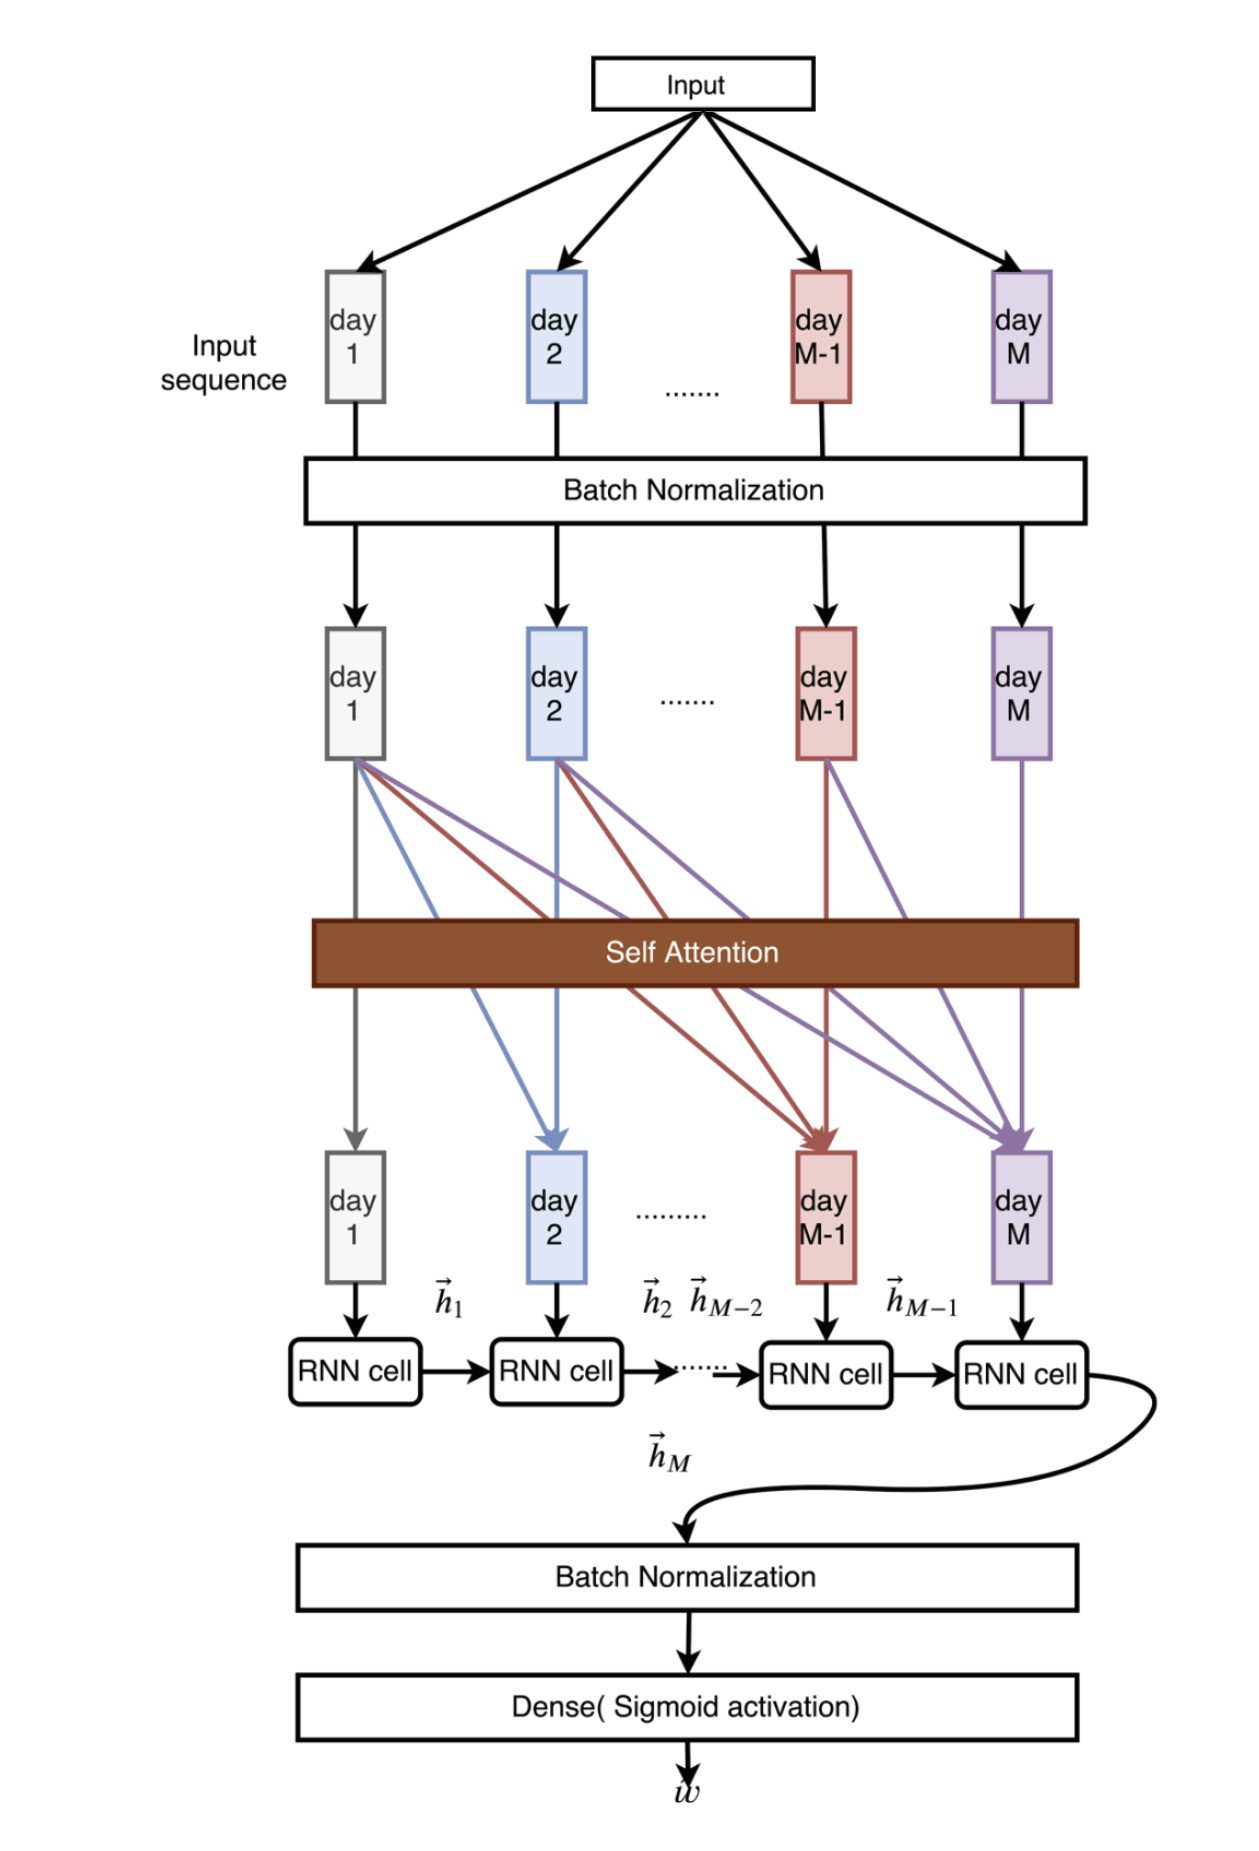
\includegraphics[width=0.8\textwidth]{./imagens/RNN_SelfAtt.png}
            \par \footnotesize Fonte: adaptado de \citeonline{cao2020delafo}.
        \end{figure}

        \begin{figure}[htp]
            \centering
            \caption{Fluxograma de redes neurais de RNN com atenção de Bahdanau.}
            \label{fig:RNN_BauhAtt}
            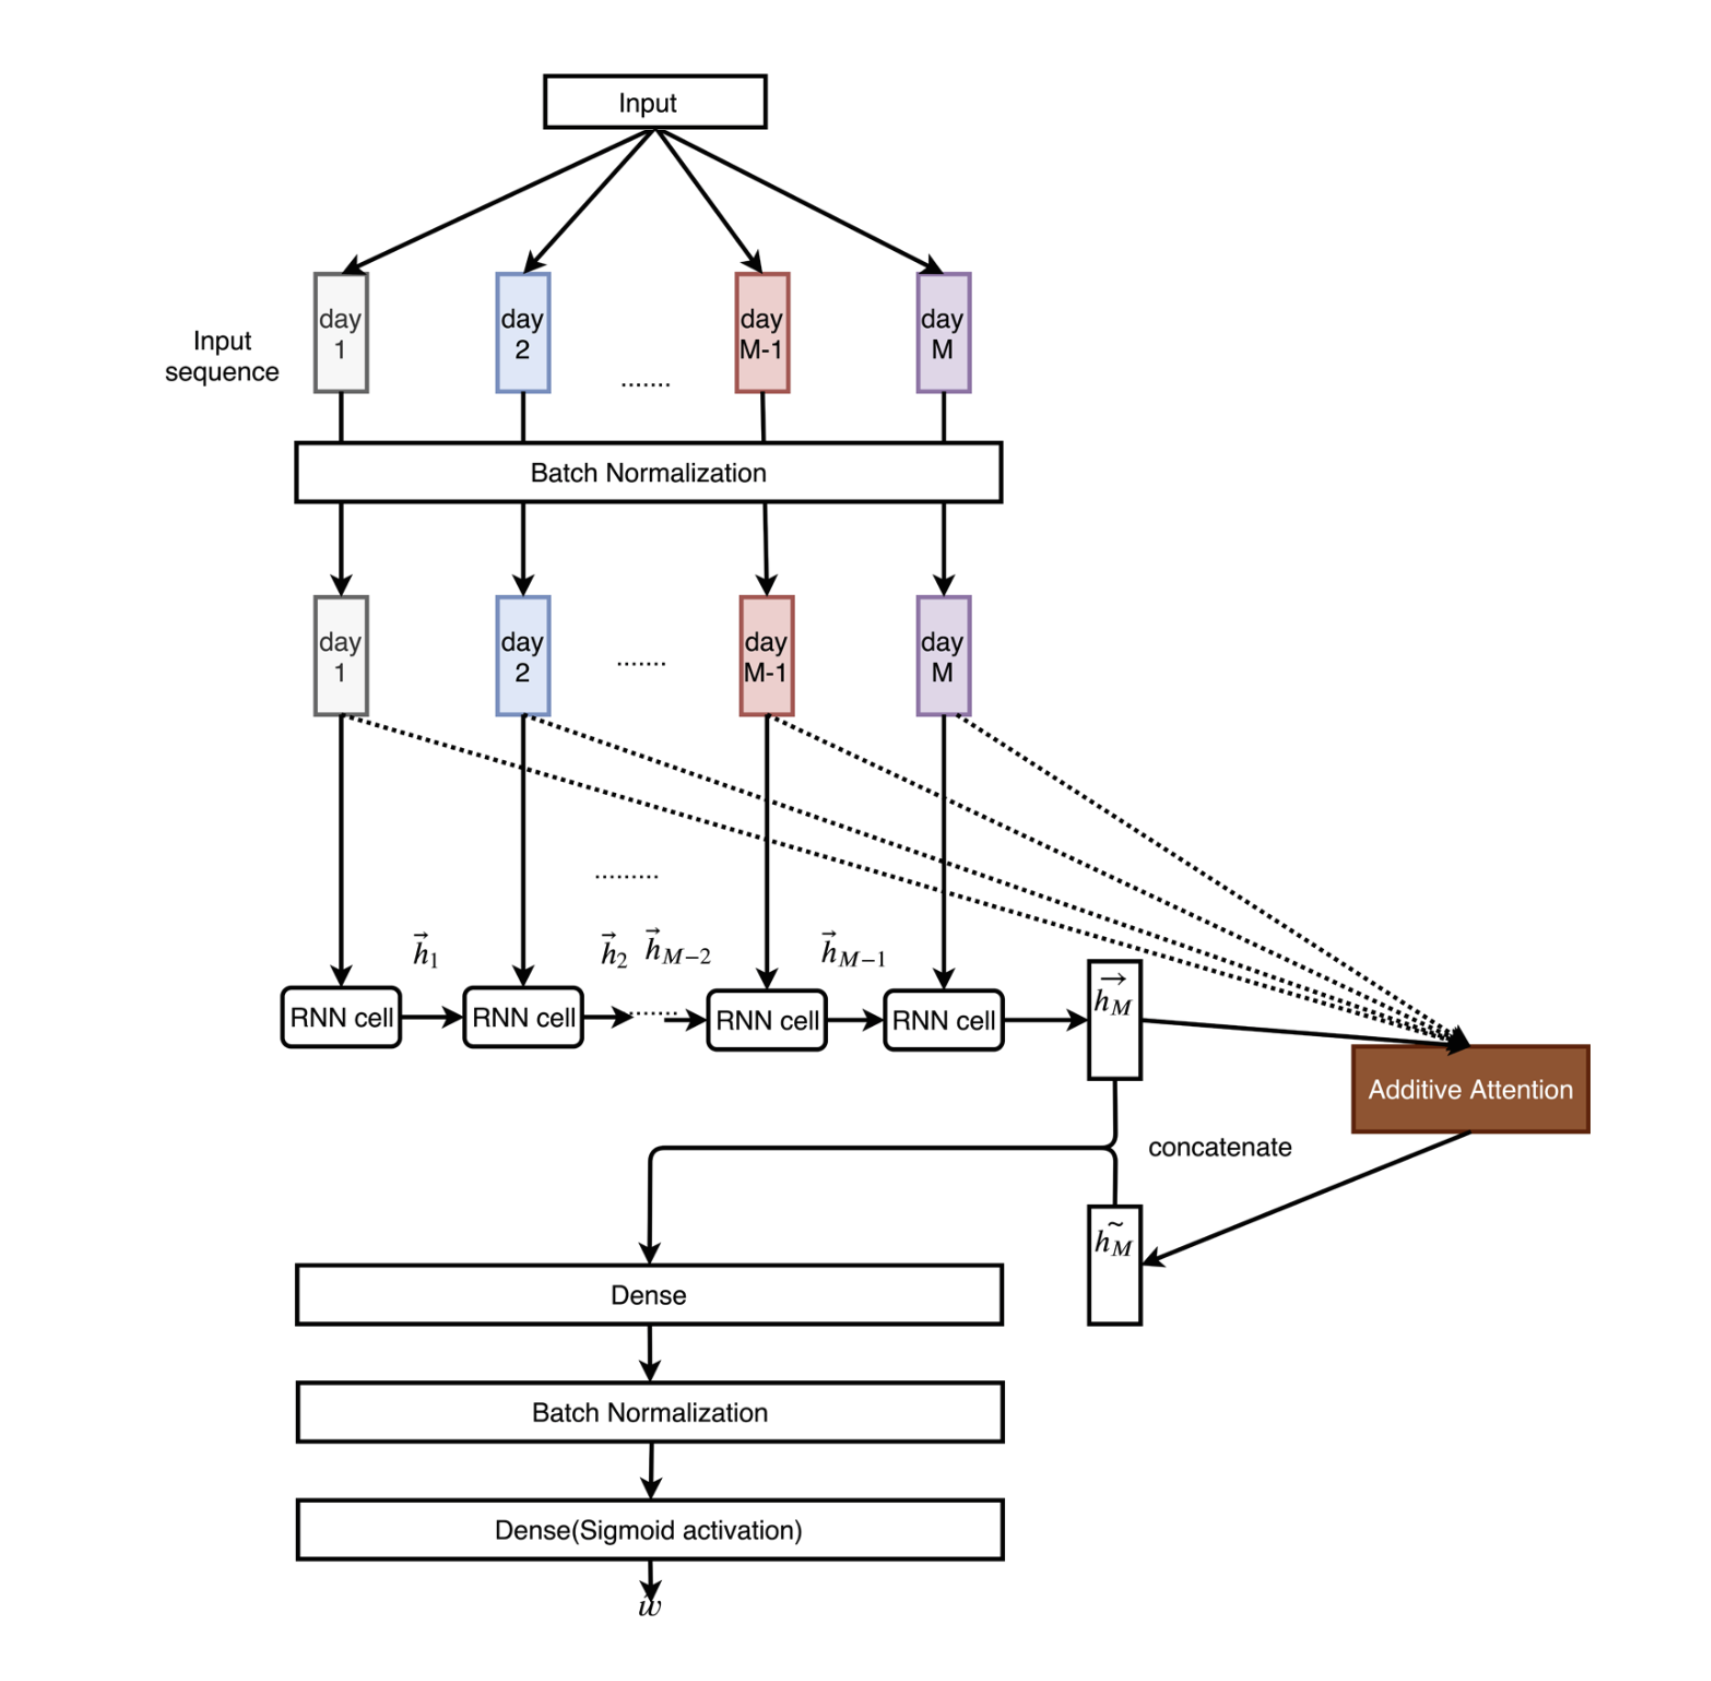
\includegraphics[width=0.95\textwidth]{./imagens/RNN_AddAtt.png}
            \par \footnotesize Fonte: adaptado de \citeonline{cao2020delafo}.
        \end{figure}

        \ipar As estruturas propostas, consideram a entrada de séries temporais dos valores dos ativos em conjunto com a taxa livre de risco e o índice de mercado. Estes valores passam por uma normalização com o objetivo de reduzir o custo computacional e melhorar a convergência do modelo. A normalização aplica uma transformação para manter os valores com média zero e desvio padrão próximo a um. No método de auto atenção, é aplicado o mecanismo de atenção antes de inserir os dados nas redes neurais recorrentes, enquanto para o método de atenção de Bahdanau, é aplicado o mecanismo de atenção após a rede neural recorrente com os dados de entrada, e a camada de contexto concatenada com a camada do último estado da rede neural recorrente. A rede neural recorrente é utilizada para capturar a dependência temporal dos dados, enquanto o mecanismo de atenção é utilizado para capturar a dependência entre os dados. Em seguida os dados são novamente normalizados e seguem para uma camada de redes neurais artificiais para previsão do índice Sharpe, isto é, a predição da melhor carteira no período. 
        
        \ipar Para os parâmetros da rede neural, é considerado o otimizador Adam, função de perda \textit{categorical cross entropy} e métrica de avaliação de acurácia. As camadas de redes neurais recorrentes, LSTM e GRU, apresentam 32 unidades ocultas e função de ativação sigmoidal com regularização $L_{2}$. A camada de atenção de Bahdanau apresenta 32 unidades ocultas e função de ativação tangente hiperbólica. A camada de auto atenção apresenta 32 unidades ocultas, e a camada de redes neurais artificiais apresenta 32 neurons e função de ativação tangente hiperbólica com regularização $L_{2}$. A camada de saída apresenta 16 neurons e função de ativação softmax com regularização $L_{2}$. As estruturas de rede neuraais são apresentadas na figura \ref{fig:model_lstm_BauhAtt} e \ref{fig:model_lstm_SelfAtt}.


        \begin{figure}[htpb]
            \centering
            \caption{Estrutura de rede neural LSTM com atenção de Bahdanau.}
            \label{fig:model_lstm_BauhAtt}
            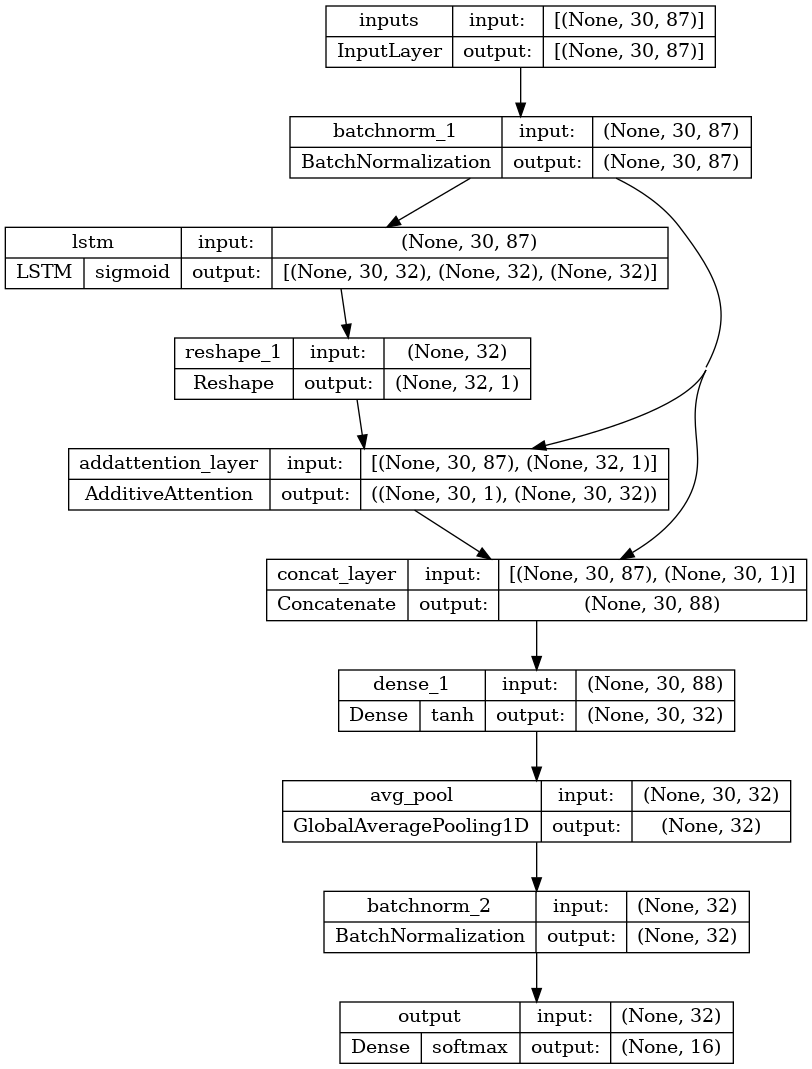
\includegraphics[width=0.8\textwidth]{./imagens/model_lstm_BauhAtt.png}
            \par \footnotesize Fonte: próprio autor.
        \end{figure}

        \begin{figure}[htp]
            \centering
            \caption{Estrutura de rede neural LSTM com auto atenção.}
            \label{fig:model_lstm_SelfAtt}
            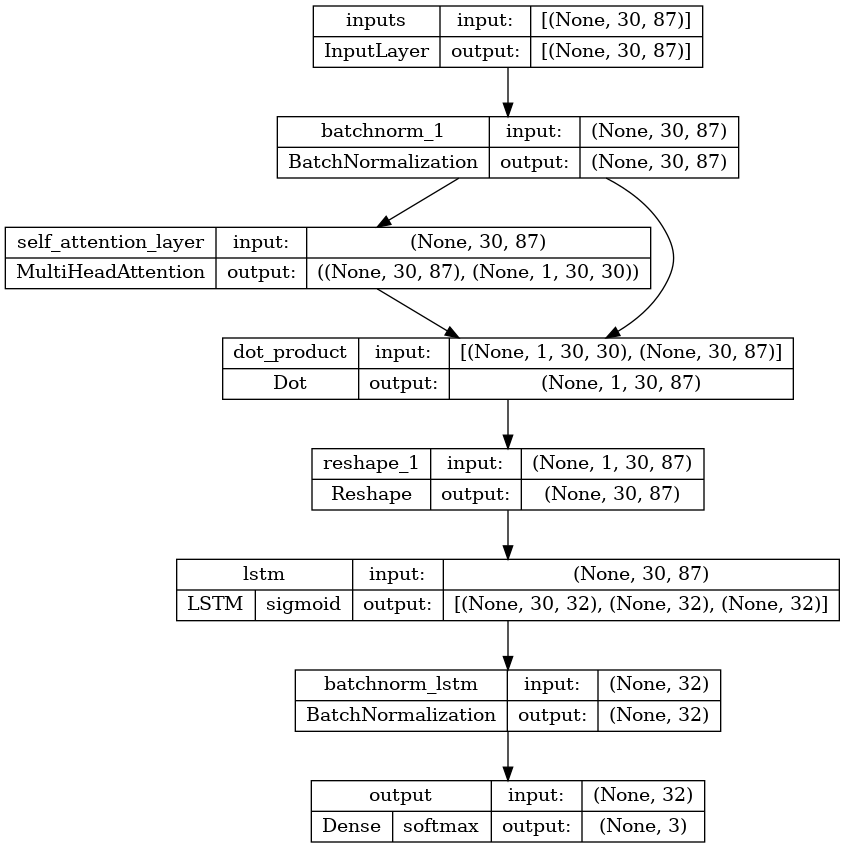
\includegraphics[width=0.8\textwidth]{./imagens/lstm_selfatt.png}
            \par \footnotesize Fonte: próprio autor.
        \end{figure}


        \ipar Os hiperparâmetros da rede neural são ajustados com o método de Hyperband Tuning, sendo neste modelo os hiperparâmetros de taxa de aprendizagem, e as regularizações $L_{2}$ definidos para a busca dos valores ótimos de $0.0001$ a $1$ distribuídos em função logarítmica reversa. O método tem como validação a acurácia, e é considerado no máximo 30 épocas de treinamento.

        \ipar Para o treinamento da rede neural, é considerado o método de validação cruzada com lacunas, onde o conjunto de dados será dividido em 13 partes, e a cada iteração, uma parte é utilizada para validação e as demais para treinamento. A validação cruzada com lacunas é utilizada para evitar o sobre-ajuste do modelo devido a utilização de séries temporais ter dependência temporal. A figura \ref{fig:cross_validation} apresenta o método de validação cruzada com lacunas.

        \begin{figure}[htp]
            \centering
            \caption{Validação cruzada com lacunas.}
            \label{fig:cross_validation}
            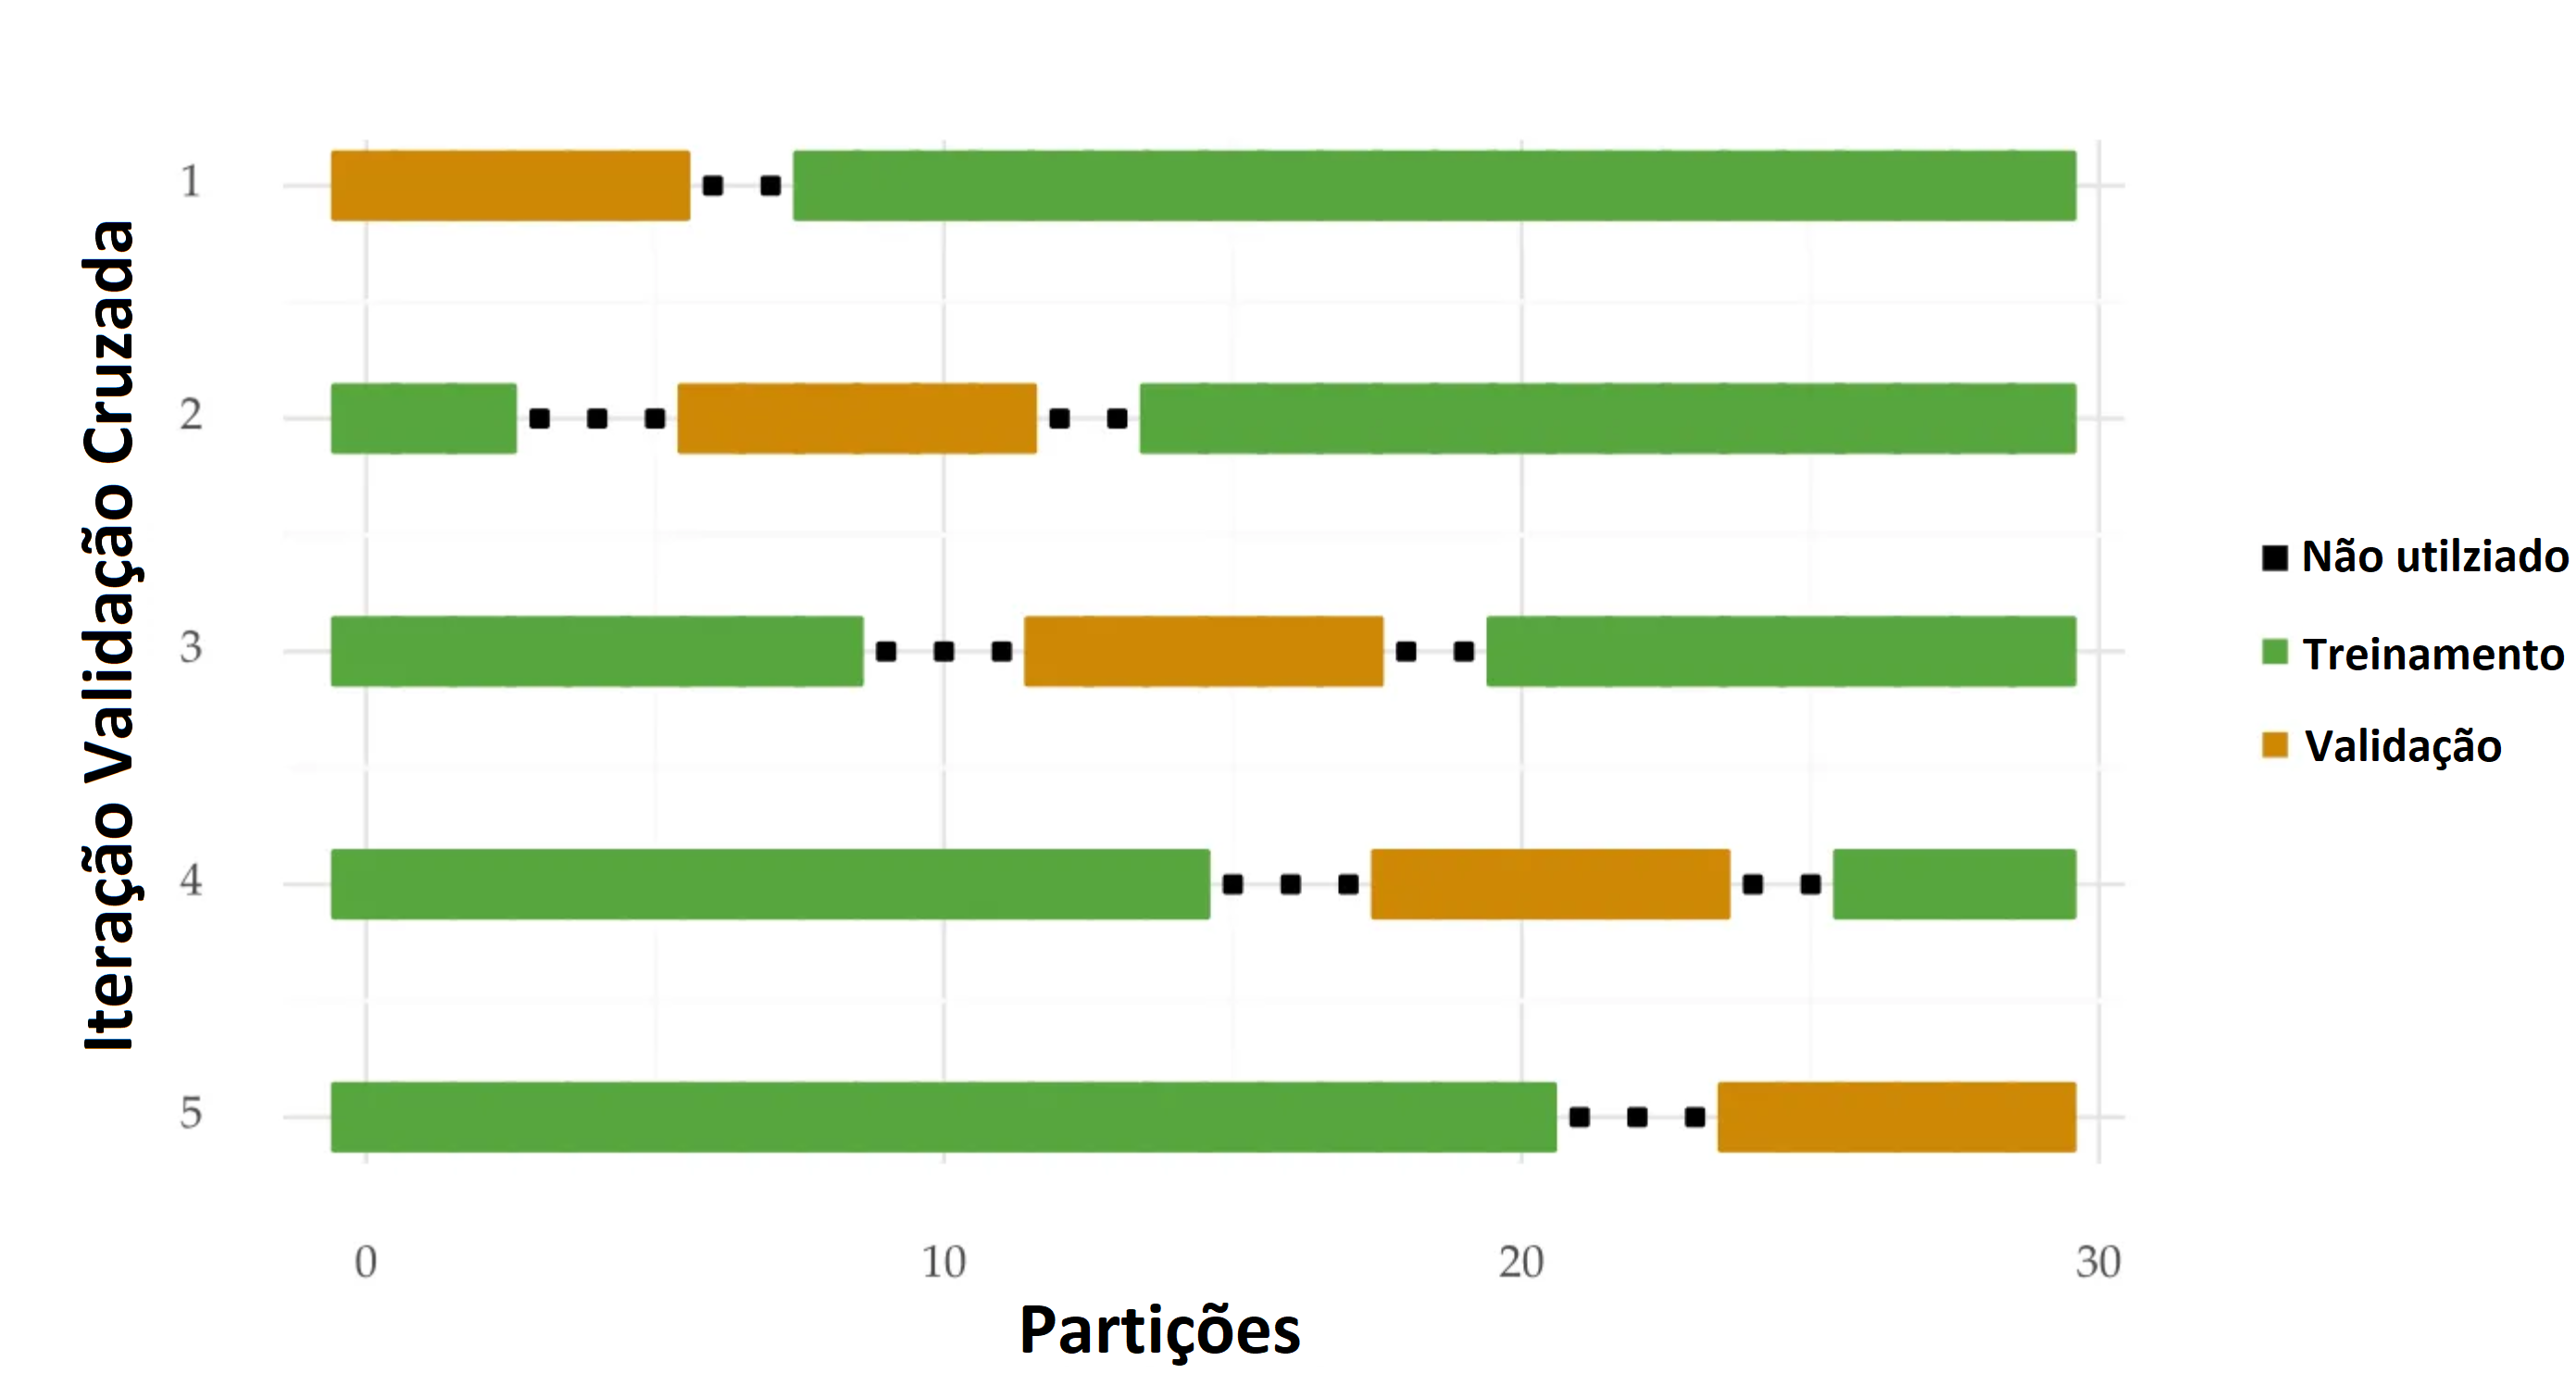
\includegraphics[width=0.8\textwidth]{./imagens/cross_validation.png}
            \par \footnotesize Fonte: \citeonline{Cerqueira2023}.
        \end{figure}

        \ipar O treinamento dos hiperparâmetros utiliza uma das partes para realizar o ajuste, enquanto para o treinamento final da rede realiza a validação em cada uma das partes considerando 100 épocas, e tamanho de lotes de 32.

        \ipar Para a validação do modelo, é considerado o período de setembro de 2018 a janeiro de 2023, resultando em 1078 dados somente ativos que compõem atualmente o índice Ibovespa, um total de 87. O modelo tem como alvo 3 carteiras otimizadas pelo índice Sharpe de forma dinâmica com parâmetros definidos de tipo de média simples e desvio padrão, e correlação para o mesmo intervalo de tempo. Os intervalos considerados são de 15, 30 e 60 dias. A carteira de referência é o \acrshort{IBOVESPA}, e a carteiras otimizadas são ajustadas diariamente. O alvo atribuído para rede neural é a escolha da carteira de maior índice Sharpe para o próximo período, sendo treinada com a aplicação das séries temporais de preço dos ativos blocos de 30 dias, isto é, os últimos 30 dias de preços são utilizados para prever a melhor carteira para o próximo dia.

    \subsection{Validação de modelos}
        % Rolagem de resultados de previsão de redes neurais, e comparação com valores de referencia, o valore de mercado (ibov), portfólio fixo após otimização no ínicio de período, portfólio dinâmico com ajuste regular, e portfólio dinâmico com ajuste de redes neurais. 

        \ipar Para a teste dos modelos, as redes neurais são treinadas novamente para todo o período de validação e são realizados as predições no período de teste, que é o intervalo no ano de 2023 até o mês de julho, resultando em 120 dados. Desta maneira, compara-se as 3 carteiras otimizadas pelo índice Sharpe para treinamento das redes neurais, com as carteiras dinâmicas aplicando a utilização do modelo de redes neurais para previsão do índice Sharpe, inclui-se também para a análise, a carteira de referência de mercado, o \acrshort{IBOVESPA}. Desta maneria, é feito a rolagem dos dados no período para avaliação das redes neurais.

\pagebreak
